\documentclass[tikz,border=2pt]{standalone}
\usepackage{amsmath,amssymb}
\usepackage{tikz}
\usetikzlibrary{arrows.meta}

\begin{document}
% atan2(y, x) returns the full angle of the point (x, y), quadrant included, in (-pi, pi];
% plain arctan(y/x) cannot tell (x, y) from (-x, -y).
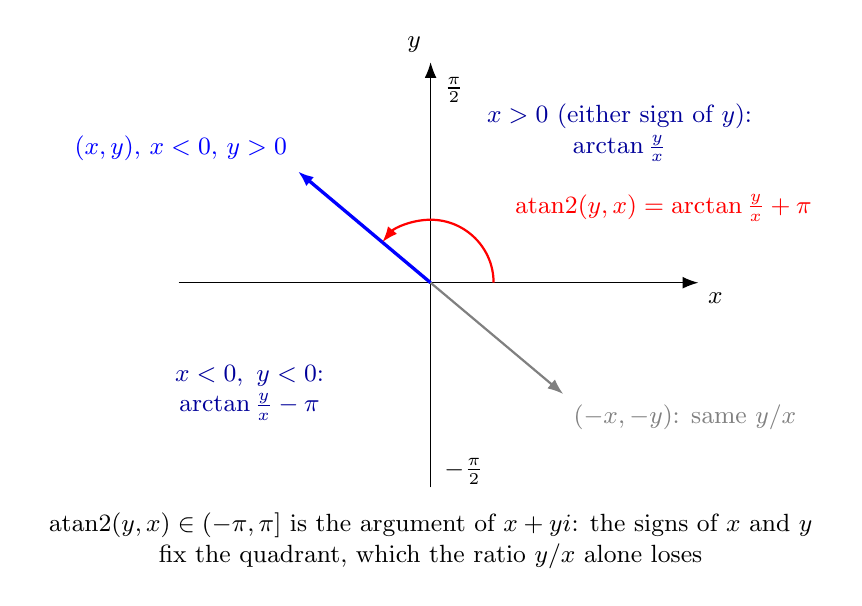
\begin{tikzpicture}[every node/.style={font=\small}, >={Latex[length=2mm]}]
	\draw[->] (-3.2,0) -- (3.4,0) node[below right] {$x$};
	\draw[->] (0,-2.6) -- (0,2.8) node[above left] {$y$};
	\draw[->, blue, very thick] (0,0) -- (140:2.2) node[above left] {$(x,y)$, $x<0$, $y>0$};
	\draw[red, thick, ->] (0.8,0) arc (0:140:0.8);
	\node[red, font=\small, anchor=west] at (0.95,0.95) {$\operatorname{atan2}(y,x)=\arctan\frac yx+\pi$};
	\draw[->, gray, thick] (0,0) -- (-40:2.2) node[below right] {$(-x,-y)$: same $y/x$};
	\node[blue!60!black, font=\small, align=center] at (2.4,1.9) {$x>0$ (either sign of $y$):\\ $\arctan\frac yx$};
	\node[blue!60!black, font=\small, align=center] at (-2.3,-1.4) {$x<0,\ y<0$:\\ $\arctan\frac yx-\pi$};
	\node[font=\small, right] at (0.05,2.45) {$\tfrac\pi2$};
	\node[font=\small, right] at (0.05,-2.4) {$-\tfrac\pi2$};
	\node[anchor=north, align=flush center, text width=10cm] at (0,-2.8) {$\operatorname{atan2}(y,x)\in(-\pi,\pi]$ is the argument of $x+yi$: the signs of $x$ and $y$ fix the quadrant, which the ratio $y/x$ alone loses};
\end{tikzpicture}
\end{document}
